\documentclass[a4paper]{article}
%\usepackage[T1]{fontenc}
\usepackage[utf8]{inputenc}
\usepackage{url}
%\usepackage{html}
%\usepackage{hthtml}
\usepackage{geometry}
\usepackage{graphicx}
\graphicspath{ {images/} }

% Comments (optional argument is author of comment)
\newcommand{\comments}[2][?]{
  \begin{quote}
    \textbf{Comment (#1):} {\em #2}
  \end{quote}
  }

% \name is for ``special names'', like procedure or variable names.
\newcommand{\name}[1]{\texttt{\hturl{#1}}}

% Just a shortcut for links where the url appears as footnote.
\newcommand{\htflink}[2]{\htmladdnormallinkfoot{#1}{#2}}

\title{Bug Insertion}
\author{Gema Rodríguez Pérez}
\date{}

\sloppy
\begin{document}
\maketitle

\begin{abstract}
This is a study about code review, the main objective in this paper is the study of when an error was caused by the previous commit, where a commit is a change to the source code submitted. For us, the previous commit is the commit immediately prior. [Literature about how a bug is introduced (the fixed bugs are introduced by the previous commits)]. However, there is not enough empirical evidence. We have conducted an observational study that englobes one hundred tickets extract from a free and open-source cloud computing software platform. The experiment was focused as a first approach to prove the premise established does not hold for all cases. The results of this study shows a trend in the data involving that non fixed bugs were introduced by the prior commit. 

\end{abstract}

\section{Introduction}

From the initial studies an implicit assumption was mentioned in which errors were caused by the previous commit as in [Kim et al., 2008] Kim, S., E. James Whitehead, J., and Zhang, Y. (2008). Classifying software changes: Clean or buggy? IEEE Transactions on Software Engineering. Where the authors introduce a new technique to classify changes into two main categories, buggy or clean. But they take on that the last commit in the line was where the responsible bug was. [Write more references]

[ Find an autor who has doubts about this ....] . Nevertheless, we doubt that this empirical evidence exists and decided to try in a particular case of OpenStack. OpenStack is an open source cloud computing platform for all types of clouds, this project was created by developers and cloud computing technologists from around the world. OpenStack is a good project to be analyzed because of their high scope and their heterogeneous nature, hundreds developers are contributing to provide an infrastructure for the world's largest brands. OpenStack has merged around 609 reviews and about 310 tickets were closed in the last week. Statistics have been provided by Bicho, a tool which retrieves and organizes information from issue tracking systems. Specifically, 69 tickets were closed in Cinder, the repository that we are analyzing, last month June. 

\begin{figure}[htb]
\centering
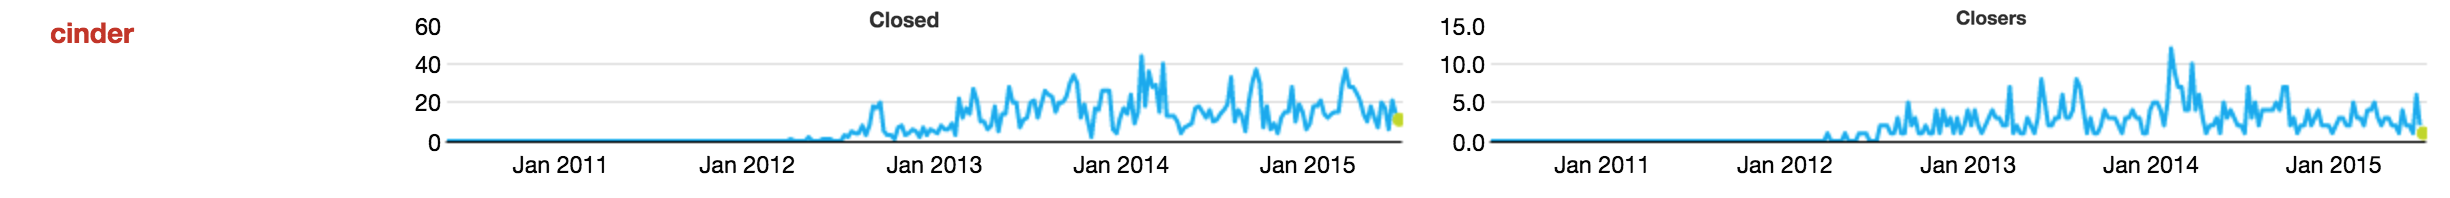
\includegraphics[width=1\textwidth]{cinder}
\caption{Evolution over the years of tickets closed and closers   } \label{fig:cinder}
\end{figure}

The study is based on an empirical experiment where one hundred tickets were extracted from an specific repository of OpenStack. Understanding the ticket as a written evolution of a bug from it is opening until it is fixed, aka bug report. The analysis of these tickets helps us to scope the principal aim, which it is none other than find the cases where we can corroborate that the error was caused by the previous commit. 

The present study answers the following research questions:
\begin{itemize}
	\item Research question 1 : Is the ticket analyzed a real bug? 
	\item Research question 2: What percentage of real bug fixes can we corroborate, in a safe way, that the antecesor change caused the error? 
	\item Research question 3: What percentage of real bug fixes can we corroborate, in a safe way, that the antecesor change did not cause the error? 
	\item Research question 4: How can we classify the antecesor changes? 
\end{itemize}

This paper describes our empirical experience to classify the percentage times that the actual
teorema is correct, is not correct and is difficult to give a proper classification. We discuss how to extract data from a specific repository and classify them as well as how the experiment was done in Section 2. The research questions are answered in section 2.1 y 2.2. Section 3 explains some of the threats that our experiment is exposed to, the intrinsic characteristics and the extrinsic characteristics. Section 4 closes with the conclusions of this study. ?
\section{The experiment}

We have carried out an empirical experiment where one hundred tickets were analyzed. These tickets were taken randomly from Cinder repository. Cinder is a component of OpenStack, it works as a Block Storage manipulating volumes and snapshots. Cinder has a Data Base in which the state of each volume can be found. 

OpenStack is a combination of software tools for building and managing cloud computing platforms for public and private clouds. Principally, users deploy it as an infrastructure as a service (IaaS) solution. The technology consists of many different moving parts. In particular, OpenStack has nine key components that can be identified as part of the 'core'. Officially, OpenStack community maintained these system. 

\begin{itemize}
    \item Compute (Nova) is the primary engine of an IaaS system. It is used for deploying and managing virtual machines.
    \item Object Storage (Swift) is a scalable redundant storage system for objects and files.
    \item Block Storage (Cinder) manages the creation, attaching and detaching of the block devices to servers, being able to access specific locations on a disk drive.
    \item Networking (Neutron) provides the networking capability for OpenStack managing IP addresses.
    \item Dashboard (Horizon) is the only graphical interface to OpenStack whereby administrators can gain graphical access.
    \item Identity (Keystone) provides a central directory of users mapped to the OpenStack services that administrators and users can access.
    \item  Image Service (Glance) provides virtual copies of services to OpenStack. It allows use of these images as templates when deploying new virtual machine instances. 
    \item Telemetry Service (Ceilometer) 
    \item Orchestration (Heat) helps to manage the infrastructure needed for a cloud service to run through both a REST API and a Query API.
\end{itemize}

Each one of the above has its own API to achieve integration. Furthermore, all of them have a repository where the community implements improvements; fixing bugs ... etc.

We focused in Cinder repository, which is composed of:
\begin{itemize}
    \item Cinder API: Accepts orders and routes them to cinder volume.
    \item Cinder Volume: Reacts to these requests, writing or reading the database. Furthermore, it interacts with other processes such as cinder Scheduler through the message queue. Also acts directly upon storage, providing hardware or software.
    \item Cinder Scheduler: Selects the node to storage and volume where created.
\end{itemize}

The experiment consists of two stages in which two different persons with knowledge of programming working in parallel analyzed and classified the tickets. Only at the end of the two stages did these people compare the results with each other, thus reaching an agreed classification when a problematic difference was found. ?
\subsection{First Stage}
The first stage considers a classification, based on our knowledge about the ticket we have analyzed, in three groups: 1. When we are sure that the ticket it is an error. 2.When we are sure that the ticket it is not an error. 3.When we have doubts about how classify the ticket, it is hardly classifiable. Henceforth, we will refer to group 1 as 'Error', group 2 as 'Not Error' and group 3 as 'Undecided'. In OpenStack, bugs reports for a project are generally tracked on Launchpad of this project, so in our case, we extracted the bugs reports from Launchpad Cinder at https://bugs.launchpad.net/cinder. Bugs reports with different status' are being found at this Launchpad, but we only are interested in tickets whose states are 'Fix Committed' or 'Fix Released' because only in these cases the changes in the code are visible. Each ticket has an id unique at Launchpad, and with this id we can see all the information about the bug. 


First of all, we must be clear in what we will analyze from the ticket that will help us to classify them. We must carefully read the title and the description of the ticket as well as the title of the commit which fixed the patch, because this is where we will obtain important information to decide to which group it belongs. Each ticket has an id unique at Launchpad, we will refer to it as 'n\_ticket', and with this id we can see all information about the bug at  \url{https://bugs.launchpad.net/cinder/+bug/n_ticket}. The title of the commit can, sometimes be found in the same link under the comment 'Fix merged to cinder (master)'. OpenStack provide us a Web interface for the Gerrit Code Review system to see proposed changes, and review them at \url{https://review.openstack.org/ }, specifically we will find this code review to each 'n\_ticket' at \url{https://review.openstack.org/#/c/n_review}, where 'n\_review' is the review unique id of each 'n\_ticket'. In the review code all the information about the patch that fixed the bug is shown.

We need to define certain criteria that must be followed in case of doubt about it being a bug or not. We have based the answer on the following criteria: 

\begin{itemize}
    \item Are there only test files? It is not an error. Our criteria indicate that test files will not be analyzed because we consider these files indispensable when a feature is implemented. With a test file the working order of the program is checked, in a way to give consistency to the program. A bug in the code, implicates there being a bug in the test file, provided that the test has been implemented. So, we are not interested in these files. 
    \item Does the title of the ticket describe a new feature? It is not an error. New features are not considered errors, because there is no failure. The optimization, deletion of a dead code or new characteristics to users are involved here. 
    \item Does the title of the ticket describe the program as not working as expected? It is an error. Sometimes the error is not in a main function which prevents Cinder from working, because a developer has considered it an important error, although not relatively important. But it is not working as he/she expected. 
    \item Does the title of the ticket describe that updates are required? It is an error. We consider all tickets that require updating as errors, because if it is not updating Cinder is not operating as expected and will cause errors. 
\end{itemize}

Sometimes we are unable to answer all the questions due to having insufficient data or because of the complexity of the issue, in this case, the ticket will be classified into the 'Undecided' group. 

At this moment, we are ready to answer the request 1 showing a graph where a percentage of the tickets are in each of three groups mentioned before showing. 

\begin{figure}[htb]
\centering
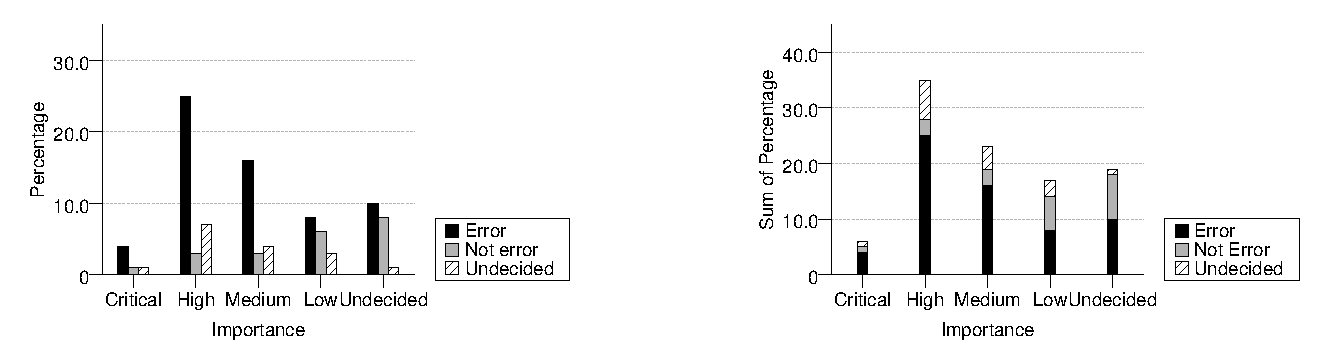
\includegraphics[width=1\textwidth]{firstStage}
\caption{Percentage of each group depending on the importance} \label{fig:firstStage}
\end{figure}

In figure ~\ref{fig:firstStage} is shown a classification of three groups which depend on the importance of label that the developers into Cinder had given to ticket.

\subsection{Second Stage}

In the second stage, we only focused in the analysis of 'Error' group. Therefore, we are committing an error in the final results due to some errors being lost when we discard the 'Undecided' group because probably in this group there are some bugs that we haven't  classified as such. In fact, this is not very important because the percentage of that group is only 16\% and the final results won't have relevant changes if we considered them. So, we decided to assume that error. 

Now the more difficult part begins. Commits will be focused on, having to identify which lines have been removed, modified or added in each of them. Also we should know in which files are the answers to the question about who is responsible. 

Sometimes, after having read the description of the ticket, we know if the ticket is an upgrade error. In this case, according to our criteria nobody is responsible for the evolution of the code. Therefore, if an update is necessary, despite being an error there is no commit responsible for the bug. In other cases, after the description we can conclude that we are unable to identify a responsible commit, because the ticket includes more than one component within OpenStack and although it has been opened in Cinder could have been closed in another repository that belongs to another component of OpenStack. Therefore we do not have a review where we analyze the code and identify the commit responsible.

If the ticket is not in any of the above situations, we have to analyze some characteristics of the commit as the kind of code it is, the number of commits involved and the number of folders modified by the fix commit. There is a free and open source distributed version control system called Git that provides us with several helpful commands for the analysis in the code review. 

Firstly we have cloned locally the Cinder repository using the 'git clone'. Then once we have chosen a ticket, extract the id of the fix commit and the id of parent commit from a web of Gerrit as well as the name of the files involved. We use 'git checkout id commit' to change between different status of these files, beginning with the id of the fix commit to obtain all characteristics mentioned before. So, using 'git blame file' command in our local repository, we find what revision and author last modified each line of a file, we save the output in a file. Then, we changed branch into the parent commit and did the same to later compare both files. 

Continuing with the methodology of the experiment, we have assumed there are three kinds of codes depending on the character of the lines, which are on the involved files. 

\begin{enumerate}
    \item New Code: When every change was executed, lines were added to each of the files.
    \item Deleted Code: When every change was  executed, there were deleted lines in each of the files.
    \item Modified Code: When the previous two codes are combined. This is the most common type of code as we can see in figure~\ref{fig:kindOfcode}
\end{enumerate}

\begin{figure}[htb]
\centering
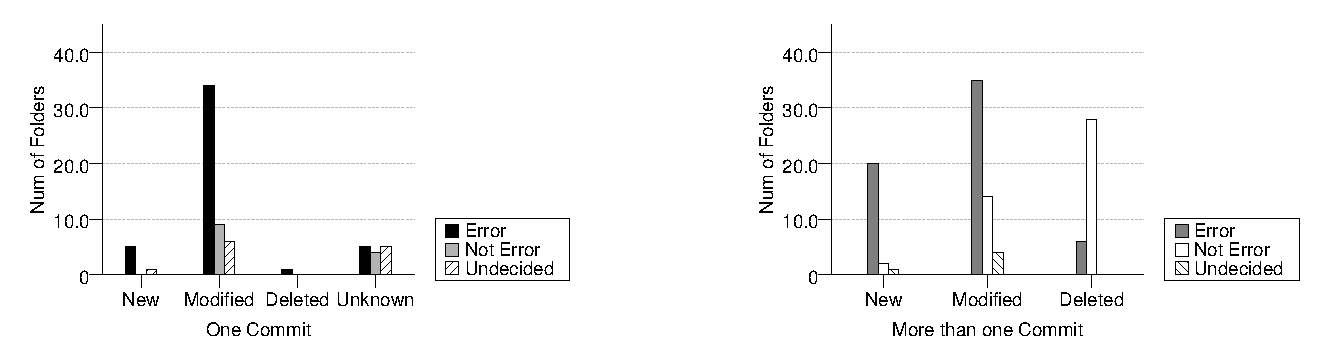
\includegraphics[width=1\textwidth]{kindOfcode}
\caption{Number of folders in each group depend on type of code} \label{fig:kindOfcode}
\end{figure}

Furthermore, we can obtain the number of lines which have been added or deleted. See in figure\ref{fig:linesOfcode}

\begin{enumerate}
    \item Number of added lines: Are the number of lines in a file ,which have been added in the actual commit (commit2) with respect to the previous commit (commit1).   
     \item Number of deleted lines: Are the number of lines in a file, which have been deleted in the actual commit with respect to the previous commit.
     \item Number of modified lines: Are the sum of the number of added lines and the number of deleted lines.
\end{enumerate}

\begin{figure}[htb]
\centering
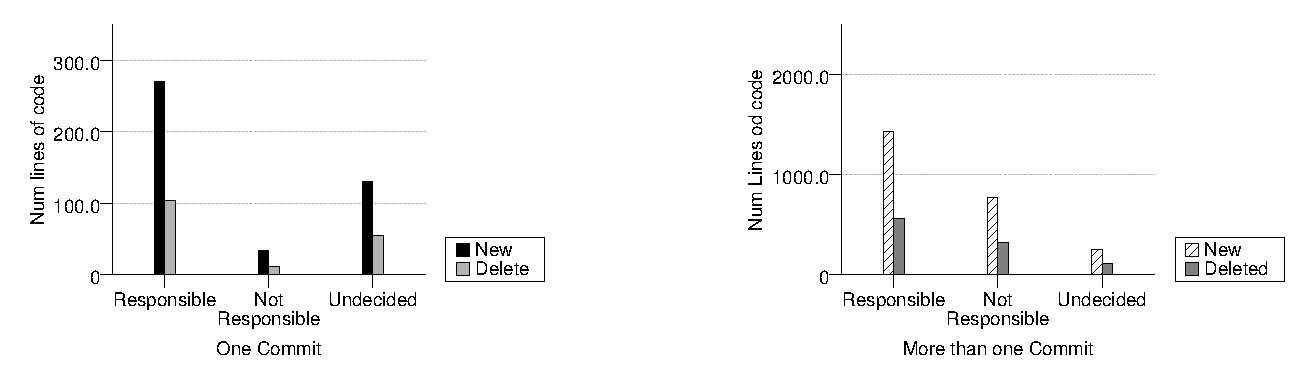
\includegraphics[width=1\textwidth]{linesOfcode}
\caption{Responsibility of each commit depend on nature of lines} \label{fig:linesOfcode}
\end{figure}


According to our experience analyzing these 100 tickets, the modified code and the deleted code are better than the new code because we have a limited reference as to where the application was failing. But, identifying the modified code is really difficult because the same lines could be in both files but located differently. So, we have been careful with this, and have checked it manually. We use 'diff -B file1 file2' command to display line\-by\-line difference between two files, the option \'-B' meaning ignore blank lines.  Diff is an algorithm extensively explained at [Ukkonen, 1985, Miller and Myers, 1985, Myers, 1986]  which provides us several source code management systems. This tool examines both files and returns  what changes, showing the number of line, need to be made for first file and second file to match, that is, returns the differences found between them.

At this stage, we got a list with all the previous commits, which could be the responsible  for the bug. At times, we can discard some commits belonging to the previous list due to the commit only adding a blank line, added or modified commentaries, or maybe, it adds to the actual number of the version file. 

Once we have that list, we have to identify those commits responsible. When there are more than one commit implicated in the same file, not everyone has to be responsible for the commit. Therefore, comparing the status of the file, before commit and after commit, we are be able to identify those commits that are responsible and those that are not. Obtaining the percentage of the degree of involvement of each of the commits involved  classifying them according to their responsibility in:

\begin{enumerate}
    \item It is the responsible
     \item It is not the responsible 
    \item Undecided
\end{enumerate}

It is now that we are ready to answer the request 2 and request 3 showing a percentage about when the antecesor change caused the error, when the antecesor change did not cause the error, and the cases hardly classifiable. 

\begin{figure}[htb]
\centering
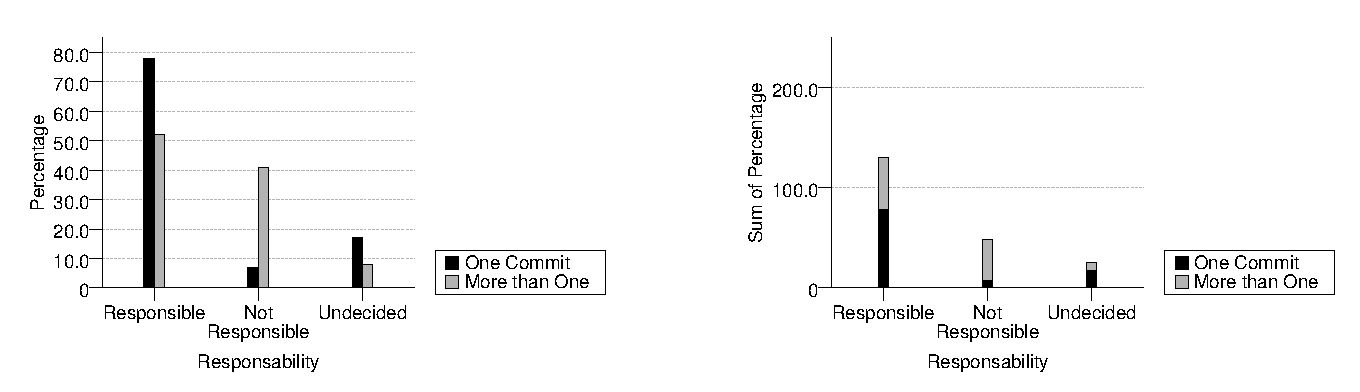
\includegraphics[width=1\textwidth]{secondStage}
\caption{Responsibility depends on number of commits implicated} \label{fig:secondStage}
\end{figure}

The figure~\ref{fig:secondStage} shows the percentage of each group depending on how many commits have been implicated in the ticket. 'More than one commits' is referring to the number of independent commits without considering tickets.

[I have another graph where the responsibility in 'More than one commit' depend on the degree of responsibility of each commit inside a ticket
\begin{figure}[htb]
\centering
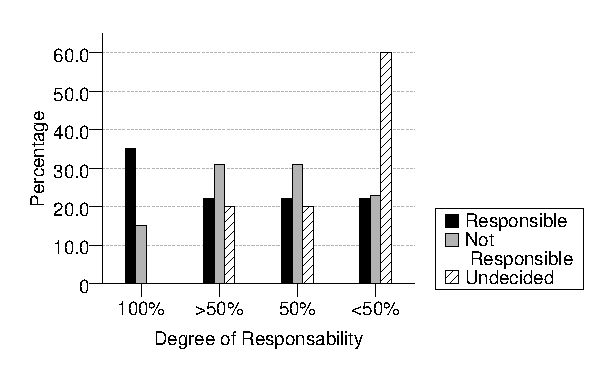
\includegraphics[width=0.5\textwidth]{prueba}
\end{figure}
]

\section{Threats to validity}

We have analyzed only 100 tickets, so our conclusions in the main are mere estimates, but along the right line. This is the first big threat. It may happen, that only with 100 seemingly random tickets, there may be a tendency, a prior unknown which matches the day of the week or month of the year.

Even so, setting aside the number of ticket analyzed, our model has a number of threats both intrinsic and extrinsic that make our model not 100\% valid. Begin with the intrinsic threats:Begin with the intrinsic threats:

\begin{itemize}
	\item Have not taken into account errors that have been classified into 'Undecided' group.
	\item There could be some lax criteria involving the subjective opinion of the reviewers. 
	\item Errors that have not been classified due to lacking of a review closed into Cinder repository.
\end{itemize}
	
Following with the extrinsic threats:
	Related to developers:
\begin{itemize}
	\item Continually mentioned bug word into description and commit of a ticket when it is not an error. It could lead the reviewer to an incorrect classification
	\item The lack of detail in the description of the ticket implies that reviewers should be experts in OpenStack. Increasing the percentage of group 'Undecided' if it does not. 
	\item The personal opinion of the developers to attach a grade of importance label could modify the figure ~\ref{fig:firstStage}.
\end{itemize}

\section{Conclusions}


\end{document}
